\documentclass[a4paper,12pt]{article}
\usepackage{jheppub}
\usepackage{taro}
\usepackage{booktabs}

\newcommand{\ab}[1]{\langle #1 \rangle}
\newcommand{\sqb}[1]{[ #1 ]}
\newcommand{\aMs}[3]{\langle #1|#2|#3]}  		% <1|2|3]
\newcommand{\aMMa}[3]{\langle #1|#2|#3\rangle}		% <1|Q_1.Q_2|3>
\newcommand{\sab}[1]{s_{#1}}
\newcommand{\twhite}[1]{\textcolor{white}{#1}}

\title{Modern amplitude techniques}

\author[a]{Taro V. Brown}

\affiliation[a]{Department of Physics, UC Davis, One Shields Avenue, Davis, CA 95616, USA }


% e-mail addresses: one for each author, in the same order as the authors
\emailAdd{taro.brown@nbi.ku.dk}


\abstract{Notes on modern amplitude techniques written as part of a research project with Jaroslav Trnka.}

\begin{document} 
\maketitle
\flushbottom
\newpage
\section{3 point amplitudes bootstrapping}
Three particle amplitudes are special since they can be completely determined by their little group scaling. From momentum conservation as well as on-shell massless kinematics we have
\begin{equation}
p_1+p_1+p_3=0\quad \Rightarrow\quad \begin{cases}
&s_{12}=(p_1+p_2)^2=\langle 12\rangle[21]=p_3^3=0\\
&s_{13}=(p_1+p_3)^2=\langle 13\rangle[31]=p_2^3=0\\
&s_{23}=(p_2+p_3)^2=\langle 23\rangle[32]=p_1^3=0\\
\end{cases}
\end{equation}
For complex momenta we can treat $\rangle p|$ and $[p|$ as independent and so for the above relations to be satisfied we need either
\begin{equation}
[12]=[23]=[13]=0\qquad\text{or}\qquad \expval{12}=\expval{23}=\expval{13}=0.
\end{equation}
Denoting the helicity of the $i$'th particle by $h_i$ the following result for the 3 point amplitude can be obtained by using the fact that under a little group scaling, the amplitudes transforms with weight according to that particles helicity:
\begin{equation}
A(1^{h_1},2^{h_2},3^{h_3})
=\begin{cases}
&\expval{12}^{h_3-h_2-h_1}\expval{23}^{h_1-h_2-h_3}\expval{13}^{h_2-h_3-h_1},\quad \sum_i h_i\leq 0\\
&[12]^{h_1+h_2-h_3}[23]^{h_2+h_3-h_1}[13]^{h_1+h_3-h_2},\qquad\: \sum_i h_i\geq 0
\end{cases}
\end{equation}
where the two cases arise because of \textit{locality}, which means that only terms that show up in a local Lagrangian such as $AA\partial A$ (from gauge term $\Tr[F^{\mu\nu}F_{\mu\nu}]$) can contribute. The condition is then there to get the correct mass dimension, meaning only amplitudes with dimensions according to local lagrangian interaction terms.
\section{Recursion Relations}\label{sec:recursion}
\textit{On-shell recursion is a systematic procedure for relating an amplitude to its
values at singular kinematics. In order to probe these kinematic configurations we define a momentum shift, which is a one-parameter deformation of
the external momenta engineered to sample various kinematic limit}. \\
%
%
A shift of the form
\begin{equation}
p_i\to p_i(z)=p_i+zq_i,~~~~z\in \mathds{C}.
\end{equation}
%
Not all momenta have to be shifted and we restrict the shifted momenta to satisfy momentum conservation as well as being on-shell
%
\begin{equation}
\sum_ip_i(z)=0,~~~~~~p_i(z)^2=0
\end{equation}
%
This implies the following for the shifts $q_i$
%
\begin{equation}
\sum_iq_i=0,~~~~~~q_i^2=q_ip_i=0.
\end{equation}
%
These conditions preserve the kinematics of the corresponding shifted amplitude
%
\begin{equation}
A\to A(z)
\end{equation}
%
We can obtain the original amplitude from the residue
%
\begin{equation}
A(0)=\oint_{z=0}\:\dd z \frac{A(z)}{z}.
\end{equation}
%
One can think of the contour integral as a deltafunction in the point $z=0$.\\
%
Using Cauchy's theorem this can be expressed as minus the sum of all the other residues 
%
\begin{equation}
A(0)=-\sum_I \Res_{z=z_I}\left[\frac{A(z)}{z}\right] +B_\infty,
\end{equation}
%
where $B_{\infty}$ is a boundary term that vanishes when $A(z)\to 0$ for $z\to \infty$. This will be another condition on what variables we shift. \\
%
If we take a subset of momenta $\{p_i\}_{\in I}$ and define the sum over these
%
\begin{equation}
P_I\equiv\sum_{i\in I} p_i,
\end{equation}
%
then we can also defined the shifted momenta $P_I(Z)$
%
\begin{equation}
P_I(z)=\sum_{i\in I} p_i(z)=P_I+zQ_I,~~~~\text{with } Q_I=\sum_{i\in I} q_i
\end{equation}
%
For simplicity we will assume $q_iq_j=0$ leading to $Q_I^2=0$. In this case $P_I(z)^2$ is linear in z
%
\begin{equation}
P_I(z)^2=(P_I+zQ_I)^2=P_I^2+zP_I Q_I=-\frac{P_I^2}{z_I}(z-z_I),
\end{equation}
%
where we have defined $z_I\equiv-\frac{P_I^2}{2P_IQ_I}$.\\
%
\textbf{For some reason} the amplitude should factorize into a product of two lower point on-shell amplitudes when $z=z_I$ and $P_I^2(z)$ goes on-shell
%
\begin{equation}
\lim_{z\to z_I}A(z)=A_L(z_I)\frac{1}{P^2_I(z)}A_R(z_I)=-\frac{z_I}{z-z_I}A_L(z_I)\frac{1}{P^2}A_R(z_I)
\end{equation}
%
Using this to take the residue at $z=z_I$
%
\begin{equation}
=-\Res_{z=z_I}\left[\frac{A(z)}{z}\right]=
\Res_{z=z_I}\left[\frac{z_I}{z(z-z_I)}A_L(z_I)\frac{1}{P_I^2}A_R(z_I)\right]
\end{equation}
%
The residue is found by multiplying by $(z-z_I)$ and setting $z=z_I$. Summing over all residues we find the amplitude
%
\begin{equation}
A(0)=\sum_I A_L(z_I)\frac{1}{P_I^2}A_R(z_I)+B_{\infty}
\end{equation}
%
The boundary contribution $B_\infty$ has no similar general expression in terms of lower-point amplitudes and the simplest way to make it vanish is by requiring  
%
\begin{equation}
A(z)\to 0,~~~~~\text{for } z\to \infty
\end{equation}
%
If this holds then 
%
\begin{equation}
A=\sum_I A_L(z_I)\frac{1}{P_I^2}A_R(z_I)=\sum_{\text{Diagrams }I} 	\raisebox{-.5\height}{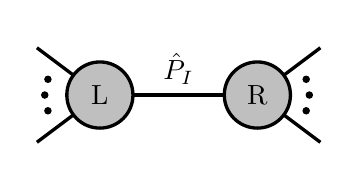
\begin{tikzpicture}[xscale=2,yscale=2]
\draw [style= very thick] (0.6,0.3) -- (1,0) node[at start, above] {};
\draw [style= very thick] (0.6,-0.3) -- (1,0) node[at start, below] {};
\draw [style= very thick] (1,0) -- (2,0) node[midway, above] {$\hat P_{I}$};
\draw [style= very thick] (2,0) -- (2.4,0.3) node[at end, above] {};
\draw [fill=black] (0.65,0) circle [radius=0.02];
\draw [fill=black] (0.67,0.1) circle [radius=0.02];
\draw [fill=black] (0.67,-0.1) circle [radius=0.02];
\draw [fill=black] (2.33,0) circle [radius=0.02];
\draw [fill=black] (2.31,0.1) circle [radius=0.02];
\draw [fill=black] (2.31,-0.1) circle [radius=0.02];
\draw [style= very thick] (2,0) -- (2.4,-0.3) node[at end, below] {};
\draw [style=very thick,fill=lightgray] (1,0) circle [radius=0.21] node[] {L};
\draw [style=very thick,fill=lightgray] (2,0) circle [radius=0.21] node[] {R};
\end{tikzpicture}}
\end{equation}
%
%
%
\subsection{BCFW-recursion}
%
A particular recursion technique used often is called BCFW recursion. In four dimensions this can be implemented in the spinor-helicity basis. Denoting the shifted variables by a hat, the shifts that we will employ are
\begin{equation}
\begin{aligned}
|\hat i]=|i]+z|j],~~~~|\hat j]=|j],~~~~|\hat i \rangle = | i \rangle,~~~~|\hat j \rangle =|j\rangle-z|i\rangle
\end{aligned}
\end{equation}
%
It can be shown that for Yang-Mills the amplitude vanishes at $z\to \infty$ for the following helicity configurations
%
\begin{align}
[i,j\rangle&~~[-,-\rangle~~[-,+\rangle~~[+,+\rangle~~[+,-\rangle\\
A_n(z)&\sim ~~\frac{1}{z}~~~~~~~\frac{1}{z}~~~~~~~~\frac{1}{z}~~~~~~~~z^3
\end{align}
%
The first 3 types of shifts will be referred to as \textit{good shifts}.
\subsection{Example of BCFW-recursion}
%
As an example, let us calculate the amplitude $A_5(1_g^+,2_g^-,3_g^+,4_g^-,5_g^-)$
Since we are dealing with an $\overline{\text{MHV}}$ amplitude we can immediately read of the good shift since the shifts
\begin{align}
|1]\to|\hat{1}]&=|1]+z|5]\\
|5\rangle\to|\hat{5}\rangle&=|5\rangle-z|1\rangle
\end{align}
will shift the amplitude by
\[
A_{5}(1^+,2^-,3^+,4^-,5^-)=\frac{[13]^4}{[12][23][34][45][51]}\to \frac{\expval{([13]+z[53])^4}}{([12]+z[52])[23][34][45]}\sim z^3
\]
While the shifts
\begin{align}
|5]\to|\hat{5}]&=|5]+z|1]\\
|1\rangle\to|\hat{1}\rangle&=|1\rangle-z|5\rangle
\end{align}
will shift the amplitude by
\[
A_{5}(1^+,2^-,3^+,4^-,5^-)=\frac{[13]}{[12][23][34][45][51]}\to \frac{[13]^4}{[12][23][34]([45]+z[41])([51]\underbrace{+z[11]}_{0})}\sim \frac{1}{z}
\]
Now since we want $A\to 0$ for $z\to \infty$ the \textit{good shift} is the second one, meaning [5] $|1\rangle$ which corresponds to a $[-,+\rangle$ shift in Elvangs notation.
%
We could have seen the good shifts by little group scaling of the amplitude since leg one has little group weight 1 and so will the amplitude under a shift will scale like z if we shift the square brackets
 The corresponding diagrams are

\begin{figure}[H]
	\centering
	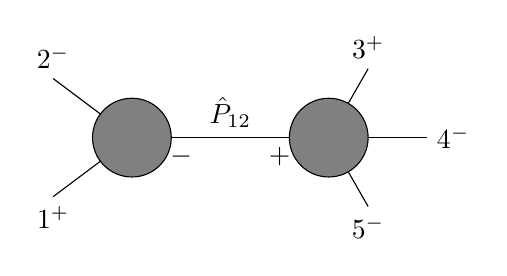
\begin{tikzpicture}[xscale=2.5,yscale=2.5]
	\draw (0.6,0.3) -- (1,0) node[at start, above] {$2^-$};
	\draw (0.6,-0.3) -- (1,0) node[at start, below] {$1^+$};
	\draw (1,0) -- (2,0) node[midway, above] {$\hat P_{12}$} node[near end, below] {$+$} node[near start, below] {$-$};
	\draw (2,0) -- (2.5,0) node[at end, right] {$4^-$};
	\draw (2,0) -- (2.2,0.35) node[at end, above] {$3^+$};
	\draw (2,0) -- (2.2,-0.35) node[at end, below] {$5^-$};
	\draw [fill=gray] (1,0) circle [radius=0.2];
	\draw [fill=gray] (2,0) circle [radius=0.2];
	\end{tikzpicture}
\end{figure}
\begin{figure}[H]
	\centering
	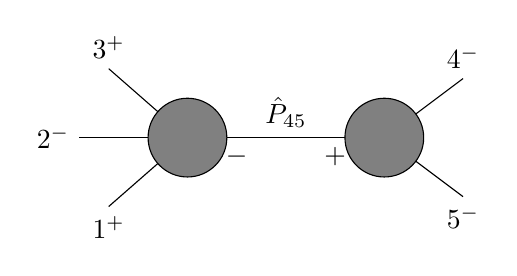
\begin{tikzpicture}[xscale=2.5,yscale=2.5]
	\draw (0.6,0.35) -- (1,0) node[at start, above] {$3^+$};
	\draw (0.6,-0.35) -- (1,0) node[at start, below] {$1^+$};
	\draw (0.45,0) -- (1,0) node[at start, left] {$2^-$};
	\draw (1,0) -- (2,0) node[midway, above] {$\hat P_{45}$} node[near end, below] {$+$} node[near start, below] {$-$};
	\draw (2,0) -- (2.4,0.3) node[at end, above] {$4^-$};
	\draw (2,0) -- (2.4,-0.3) node[at end, below] {$5^-$};
	\draw [fill=gray] (1,0) circle [radius=0.2];
	\draw [fill=gray] (2,0) circle [radius=0.2];
	\end{tikzpicture}
\end{figure}
Looking at the first diagram we see that it contains a 3-point MHV amplitude
\begin{equation}
A_3(1^+,2^-,-\hat P_{12}^-)=\frac{\expval{2\hat P_{12}}^3}{\expval{\hat 1 2}\expval{\hat P_{12}\hat 1}}
\end{equation}
Since we impose that the propagating momentum is on shell we see that
\[
0=\hat{P}_{12}=\expval{\hat 1 2}[\hat 1 2]=\expval{\hat 1 2}[1 2]
\]
So the only way to impose on shell conditions is by setting $\expval{\hat 1 2}=0$ similarly one can show that the numerator vanishes and we must have 
\[
A_3(1^+,2^-,-\hat P_{12}^-)=0
\]
which means the first diagram doesn't contribute. For the second diagram we also have a 3-point MHV amplitude, but in this case the shift is in |5] so the sub-diagram isn't zero.

We can then proceed to calculate the second diagram explicitly
\begin{align*}
A_{5}(1^+,2^-,3^+,4^-,5^-)&=A_3(\hat{P}_{45}^+,4^-,\hat 5^-)\frac{1}{P_{45}^2}A_4(\hat 1,^+,2^-,3^+,-\hat P_{45}^-)\\
&=\frac{\expval{4\hat 5}^3}{\expval{\hat P_{45}4}\expval{\hat 5\hat P_{45}}}\frac{1}{\expval{45}[45]}\frac{[\hat 13]^4}{[\hat 12][23][3\hat P_{45}][\hat P_{45}\hat 1]}
\end{align*}
Since the shift is in $[5,1\rangle$ we can remove the hat on all but the $P$'s: 
\begin{align*}
A_{5}(1^+,2^-,3^+,4^-,5^-)
&=\frac{\expval{4 5}^3}{\expval{\hat P_{45}4}\expval{5\hat P_{45}}}\frac{1}{\expval{45}[45]}\frac{[13]^4}{[12][23][3\hat P_{45}][\hat P_{45} 1]}\\
&=\frac{\expval{4 5}^3}{\expval{\hat P_{45}4}\expval{5\hat P_{45}}}\frac{1}{\expval{45}[45]}\frac{[13]^4}{[12][23][3\hat P_{45}][\hat P_{45} 1]}
\end{align*}
We can the rewrite the $\hat P$ terms in the following way:
\begin{align*}
\expval{\hat P_{45}4}[\hat P_{45}1]&=-\expval{4\hat P_{45}}[\hat P_{45}1]=\langle 4|\hat P_{45}|1]=\langle 4|4+\hat{5}|1]=\langle 4|\hat{5}|1]=-\expval{4\hat 5}[\hat 5 1]=-\expval{45}[5 1]\\
\expval{5\hat P_{45}}[3\hat P_{45}]&=-\expval{5\hat P_{45}}[\hat P_{45}3]=\langle 5|\hat P_{45}|3]=\langle 5|4+\hat{5}|4]=\langle 5|4|3]+\langle 5|\hat 5|3]\\
&=-\expval{54}[ 4 3]-\expval{5\hat 5}[ \hat 5 3]=-\expval{54}[ 4 3]=-\expval{45}[34]
\end{align*}
where we in the first terms have used the fact that $|\hat 5\rangle=|5\rangle$ and $[\hat 5 1]=[51]+z[11]=[51]$, while in the second term using $\expval{5\hat 5}=\expval{5 5}=0$. Inserting this into the amplitude we get
\begin{align*}
A_{5}(1^+,2^-,3^+,4^-,5^-)
&=\frac{[13]^4\expval{45}^3}{[12][23][45]\expval{45}^3[51][34]}\\
&=\frac{[13]^4}{[12][23][34][45][51]}
\end{align*}
which is the expected result.
\subsection{Soft limit factorization}
The soft-limit factorization for tree amplitudes is that for $k_s\to 0$ we can write an n-point amplitude as
\begin{equation}
A_n^{\text{tree}}(1,2,\dots,a,s^\pm,b,\dots,n)=\mathcal{S}(a,s^\pm,b)\times A_{n-1}^{\text{tree}}(1,2,\dots,a,b,\dots,n)
\end{equation}
where
\begin{equation}
\mathcal{S}(a,s^+,b)=\frac{\expval{ab}}{\expval{as}\expval{sb}},\qquad \mathcal{S}(a,s^-,b)=-\frac{[ab]}{[as][sb]}
\end{equation}
Here this gets us
\begin{align*}
A_{5}(1^+,2^-,3^+,4^-,5^-)=-\frac{[41]}{[45][51]}\times\frac{[13]^4}{[12][23][34][41]}
\end{align*}
which is a valid factorization of the full result.
\subsection{Co-linear limit}
In the co-linear limit for leg 1 and 2 we have the two momenta $k_1$ and $k_2$ that become parallel with intermediate momentum $k_P$. The spinors also have the following relations
\begin{align*}
&\lambda_a\simeq\sqrt{z}\lambda_P,\qquad \lambda_b\simeq \sqrt{1-z}\lambda_P\\
&\tilde\lambda_{\dot a}\simeq\sqrt{z}\tilde\lambda_P,\qquad \tilde\lambda_{\dot b}\simeq \sqrt{1-z}\tilde\lambda_P
\end{align*}
taking the amplitude we calculated in part a and shifting it in this limit gives
\[
A_5(1^+,2^-,3^+,4^-,5^-)\to \frac{z^2}{\sqrt{z(1-z)}[12]}\frac{[P3]^4}{[P3][34][45][5P]}
\]
which is the result we expected from Dixon:
\begin{equation}
A_{n}^{\text{tree}}(\dots,a^{\lambda_a},b^{\lambda_b},\dots)\to \sum_{\lambda_p=\pm}\text{Split}_{-\lambda_P}(a^{\lambda_a},b^{\lambda_b};z)A^{\text{tree}}_{n-1}(\dots,P^{\lambda_P},\dots)
\end{equation}
where
\begin{equation}
\text{Split}_{-}(a^+,b^-)=\frac{z^2}{\sqrt{z(1-z)}[ab]}
\end{equation}
%
\section{Unitarity}
\subsection{Loops in general}
\textit{Feynman rules require momentum conservation at each vertex of a Feynman diagram.At tree-level, this fixes all momenta of the internal lines in terms of the external momenta. At loop-level, momentum conservation leaves one momentum undetermined per loop and one must integrate over all such unfixed momenta. Thus in $D$-dimensions, one has a $D$-dimensional loop-integral for each loop}.
\section{Unitarity}
Take a general analytic function of some variable $x$
\begin{equation}
\begin{aligned}
f(x)&=\beta(x)+i\alpha (x)
\end{aligned}
\end{equation}
Defining the discontinuity of this function as $\text{Disc}[f(x)]=if(x+i\epsilon)-if(x-i\epsilon)$ we find as we let $\epsilon\to 0$
\begin{equation}
\begin{aligned}
if(x+i\epsilon)-if(x-i\epsilon)&=i\beta(x+i\epsilon)-\alpha(x+i\epsilon)-i\beta(x-i\epsilon)-\alpha(x-i\epsilon)\\
&=-2\left(\alpha(x)+i\beta(i\epsilon)\right)+\mathcal{O}(\epsilon^2)\\
&=-2\alpha(x)+\mathcal{O}(\epsilon)\\
&=-2\Im[f(x)]
\end{aligned}
\end{equation}
The scattering matrix is unitary
\begin{equation}
S=\mathds{1}+iT
\end{equation}
Taking
\begin{equation}
\begin{aligned}
S^\dagger S&=(\mathds{1}-iT^\dagger)(\mathds{1}-iT)=1\\ &=\mathds{1}-i(T-T^\dagger)-T^\dagger T=1\\
\Rightarrow T^\dagger T&=i(T^\dagger -T)=i\left[(\Re[T]-i\Im[T])-(\Re[T]+i\Im[T])\right]\\
&=2\Im[T]=-\text{Disc}[iT]
\end{aligned}
\end{equation}
Expanding this order by order in perturbation theory we have for instance at four and five point
\begin{equation}
\begin{aligned}
T_4&=g^2T_4^{(0)}+g^4T_4^{(1)}+g^6T_4^{(2)}\\
T_5&=g^3T_5^{(0)}+g^5T_5^{(1)}+g^7T_5^{(2)}\\
\end{aligned}
\end{equation}
with $T_n^{(L)}$ being the $n$-point gluon amplitude at $L$-loop. By inserting these into the equation for the discontinuity we find first to order $g^2$
\begin{equation}
\text{Disc}[T_4^{(0)}]=0
\end{equation}
Since we cant construct the amplitude from the product of two other amplitudes. This simply states that tree level amplitudes have no branch cuts. At order $g^4$ we have 
\begin{equation}
	\text{Disc}[T_4^{(1)}]=T_4^{(0)\,\dagger} T_4^{(0)}
\end{equation}
This is equivalent to cutting to lines in the one loop diagram and obtaining two four point tree-level diagrams with an on-shell propagator in between, which momentum obviously must depend on the loop momentum $\ell$.\\
Using the optical theorem the Discontinuity of a function is related directly to the scattering cross-section.
\section{Generalized unitarity}
When we take the momenta in the scattering amplitudes to be complex and use the unitarity method, we get \textit{generalized unitarity}. The inclusion of complex momenta opens up the possibility of cutting more than two lines. e.g. the three-point amplitudes are only non-zero for complex momenta, so for the four-point one-loop amplitude we could cut four lines and end up with a product of four three-point amplitudes.\\
In general we will in fact only be able to cut up to four lines since we need momentum conservation at the vertices as well as having the cut momentum being on-shell. This imposes one new condition for every cut, and since $\ell^\mu$ has four components we need 4 equations.
%%%%%%%%%%%%%%%%%%%%%
\section{Exterior derivatives and forms}
An $n$-form $F_{(n)}$ is a completely antisymmetric tensor 
\begin{equation}
F_{\mu_1\,\mu_2\,\mu_3\,\cdots\,\mu_n}=-F_{\mu_1\,\mu_3\,\mu_2\,\cdots\,\mu_n}=F_{\mu_3\,\mu_1\,\mu_2\,\cdots\,\mu_n}
\end{equation}
On this $n$-form, we can define an exterior derivative, which is an $(n+1)$ form:
\begin{equation}
\dd F_{\mu_1\,\mu_2\,\mu_3\,\cdots\,\mu_n}=(n+1)\partial_{[\mu_1}F_{\mu_2\,\mu_3\,\cdots\,\mu_n]},
\end{equation}
where the square brackets just mean that we antisymmetrize in the indices, e.g.
\begin{equation}
\begin{aligned}
\dd F_{\mu\nu}=&\frac{(1+1)}{2!}\left(\partial_\mu F_\nu-\partial_\nu F_\mu\right)\\
=&\partial_\mu F_\nu-\partial_\nu F_\mu,\\ \dd F_{\mu\nu\rho}=&\frac{(2+1)}{3!}\left(\partial_\mu F_{\nu\rho}-\partial_\mu F_{\rho\nu}-\partial_\nu F_{\mu\rho}+\partial_\nu F_{\rho\mu}-\partial_\rho F_{\nu\mu}+\partial_\rho F_{\mu\nu}\right)\\
=&\partial_\mu F_{\nu\rho}+\partial_\nu F_{\rho\mu}+\partial_\rho F_{\mu\nu}
\end{aligned}
\end{equation}
Furthermore we have the property
\begin{equation}
\dd^2 F=0
\end{equation}
And the following nomenclature
\begin{itemize}
\item \textit{Exact form}: if we can write $\qquad F=\dd G$
\item \textit{Closed form}: if $\qquad \qquad \qquad ~~~ \dd F=0$
\item $\Rightarrow$ All exact forms are closed.
\end{itemize}
We also define the wedge product of forms. Given two forms $F_{(n)}$ and $G_{(m)}$, we can define the $n+m$ form $F\wedge G$
\begin{equation}
(F\wedge G)_{\mu_1\,\cdots\,\mu_{n+m}}=\frac{(n+m)!}{n!m!}F_{[\mu_1\,\cdots\,\mu_n}G_{\mu_{n+1}\,\cdots\,\mu_{n+m}]}
\end{equation}
For instance
\begin{equation}
\begin{aligned}
F_\mu\wedge G_\nu=&\frac{(1+1)!}{1!1!}\left(F_\mu G_\nu-F_\nu G_\mu\right)\\
=&2[F_\mu,G_\nu]
\end{aligned}
\end{equation}
Lastly we can define the \textit{Hodge dual}, as the $(D-n)$-form
\begin{equation}
^{*}\hspace*{-0.1cm}F^{\mu_{n+1}\,\mu_{n+2}\,\cdots\,\mu_{D}}=\frac{1}{n!}F_{\mu_1\,\mu_2\,\cdots\,\mu_n}\epsilon^{\mu_1\,\mu_2\,\cdots\,\mu_n\,\mu_{n+1}\,\mu_{n+2}\,\cdots\,\mu_D}
\end{equation}
Using this notation we can write the source-less Maxwell equations as:
\begin{equation}
\begin{aligned}
\dd F&=0\\
\dd \hodge F&=0
\end{aligned}
\end{equation}
\newpage
\section{Projective spaces}
We will start by considering $\mathds{P}^2$. Any geometric questions that do not involve distance are best thought of projectively. All lines that intersect the origin in $\mathds{R}^3$ can be though of as points crossing a plane
\begin{figure}[H]
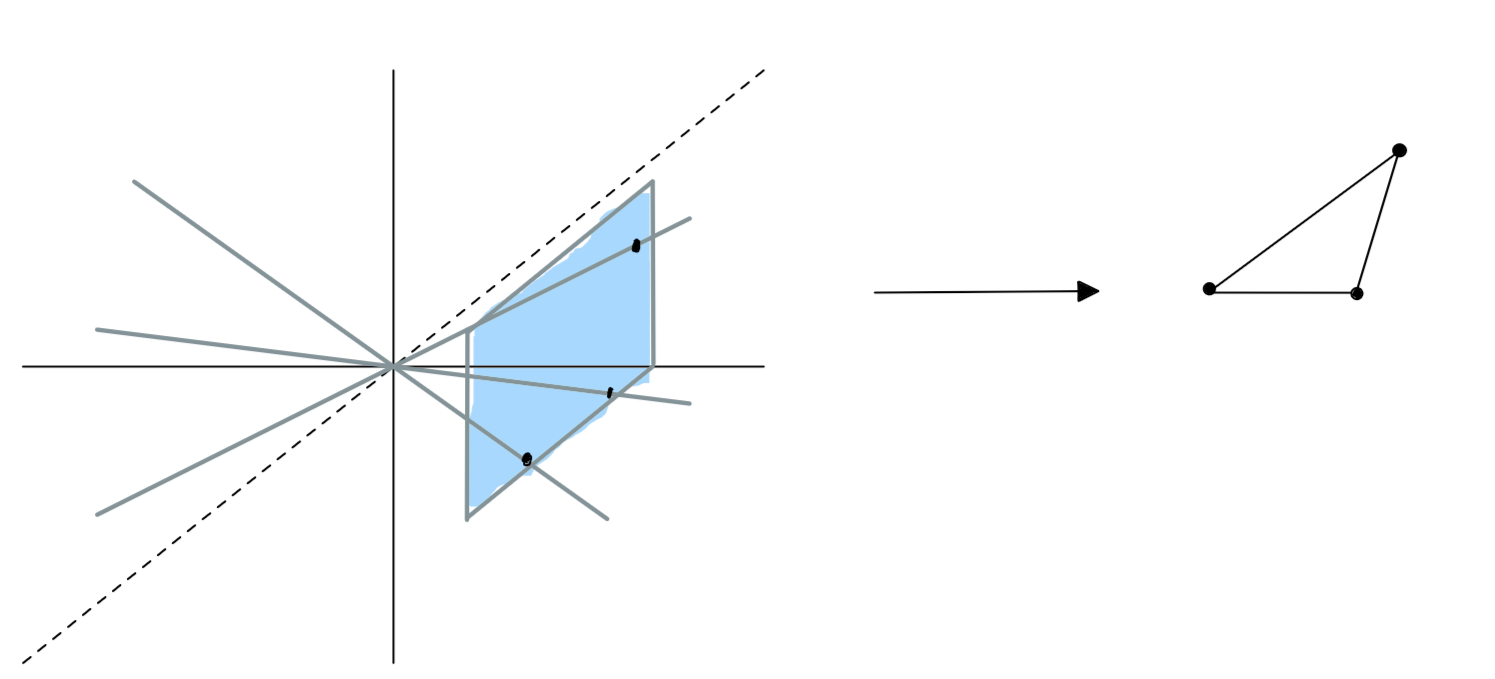
\includegraphics[width=15cm]{projec.PNG}
\end{figure} 
If we denote the points by $Z_I=\begin{pmatrix}Z_0 \\ Z_1 \\ Z_2
\end{pmatrix}$ these can always be rescaled by some factor $t$ while still preserving the geometry of the points in the plane. This means that we really have two degrees of freedom per point (which should not surprise since we have a plane), so that $Z_I=\begin{pmatrix} 1\\ x_1 \\ x_2
\end{pmatrix}$. The space has an SL(3) $=$ Translations + $\underbrace{\text{Rotations}}_{\text{SL}(2)}$ symmetry, meaning all symmetries that map straight lines to straight lines. 
\\
The only invariant tensor is $\epsilon_{IJK}$.
\\
\textbf{Example: straight line}
A straight line obeys the following equation
\begin{equation}
ax+by+c=0
\end{equation}
This can be written using the $Z_I$ variables
\begin{equation}
Z_I=\begin{pmatrix}
	1\\ x\\ y
\end{pmatrix},\qquad \qquad W^I=\begin{pmatrix}
c \\ a \\ b
\end{pmatrix},\qquad \qquad Z_I W^I=0
\end{equation}
where $W$ is a line. Take e.g. $Z^1=\{1,x^1,y^2\}=\{1,1,0\}$ and $Z^2=\{1,x^2,y^2\}=\{1,10,10\}$.
%\begin{equation}
%\begin{aligned}
%W_1&=\epsilon_{1JK}Z^1_J Z^2_K=Z^1_2Z^2_3-Z^1_3Z^2_2=x_1y_2-x_2y_1\\
%W_2&=\epsilon_{2JK}Z^1_J Z^2_K=-Z^1_2Z^2_3+Z^1_3Z^2_1=-y_2+y_1\\
%W_3&=\epsilon_{3JK}Z^1_J Z^2_K=Z^1_2Z^2_2-Z^1_2Z^2_1=x_2-x_1\\
%\end{aligned}
%\end{equation}
%this gives the following line
We check that this gives the expected result
\begin{lstlisting}
In[403]:= ClearAll["Global`*"]

(*Below we define two points from which we then find the line*)

In[404]:= Z1 = {1, x1, y1};
Z2 = {1, x2, y2};
a = (y2 - y1)/(x2 - x1);
W = Z1 . LeviCivitaTensor[3] . Z2;
s = Collect[Solve[W . {1, x, y} == 0, y], x][[1]][[1]];
Equal @@ s;
y = (x (y1 - y2))/(x1 - x2) + (-x2 y1 + x1 y2)/(x1 - x2);

In[411]:= (*Testing against the usual formula*)
x1 = 1; x2 = 10; y1 = 0; y2 = 10;
yy = a x + (y2 - a x2);
yy == y

Out[413]= True
\end{lstlisting}
Similarly the point where two lines cross is given  by \begin{equation}
Z_I=\epsilon_{IJK}W_1^JW_2^K
\end{equation}
\section{Polytopes}
Let us define the five-bracket
\begin{equation} \label{eq:fivebracket}
[i,j,k,l,m]\equiv \frac{\delta^4(\chi_{i\,A}\expval{jklm}+\text{ cyclic })}{\expval{ijkl}\expval{jklm}\expval{klmi}\expval{lmij}\expval{mijk}}
\end{equation}
with $\expval{ijkl}\equiv\epsilon_{IJKL}Z^{I}_{i}Z^{J}_{j}Z^{K}_{k}Z^{L}_{l}$ and the $Z_i^I$'s are the bosonic component of the momentum supertwistors $Z_i^I=(\ket{i},[\mu_i|)$. One can write the five-bracket completely in terms of bosonic parts by introducing a five vector $\mathsf{Z}_i^\mathcal{I}$,
\begin{equation}
	\mathsf{Z}_i^\mathcal{I}=\begin{pmatrix} Z_i^I\\\chi_i\cdot \psi
	\end{pmatrix},~~~~~~~\mathcal{I}=1,\dots,5
\end{equation}
with the $\psi$ being an auxiliary Grassmann valued field. The five-bracket can then be written only in terms of the five-vectors by integrating out the fermionic auxilary field.
\begin{equation}
[i,j,k,l,m]=\frac{1}{4!}\int \dd^4\psi \frac{\expval{ijklm}^4}{\expval{0ijkl}\expval{0jklm}\expval{0klmi}\expval{0lmij}\expval{0mijkl}}
\end{equation}
where we have introduced the auxiliary reference spinor 
\begin{equation}
	\mathsf{Z}_0^\mathcal{I}=\begin{pmatrix}
0\\0\\0\\0\\1
	\end{pmatrix}
\end{equation} 
Focusing on the integrand, it is invariant under $	\mathsf{Z}_i^\mathcal{I}\to 	t_i\mathsf{Z}_i^\mathcal{I}$ and hence appear projectively which means they can be thought of as points in $\mathds{CP}^4$ with the reference vector introduced being the only thing that breaks projective invariance. This is similar to the map between the dual momentum coordinates and the momentum twistors
\begin{equation}
y^2_{ij}=\frac{\expval{i-1,i,j-1,j}}{\expval{I_0,i-1,i}\expval{I_0,j-1,j}},\qquad I_0^{IJ}=\begin{pmatrix}
0 & 0 \\
0 & \epsilon_{\dot a \dot b}
\end{pmatrix}
\end{equation}
where the $I_0$ is known as infinity twistor that is inserted to break SL(4) conformal invariance and gives a definition of distance. The fact that the reference spinor appears five times in equation \eqref{eq:fivebracket} is analogous to how $I_0$ appears twice to give the distance between $i$ and $j$, and can be regarded as giving the volume of a simplices. 
\subsection{Definitions and examples}
\textit{Simplex}: Generalization of the notion of a triangle or tetrahedron to arbitrary dimensions
\\\\
\textit{n-simplex}: Convex hull of a set of $n+1$ points. E.g. 2-simplex is a triangle.
\\\\
\textit{Polygon}: Triangle, quadrilateral, pentagon etc.
\\\\
\textit{Tetrahedron}: Solids with polygons on each face, e.g. cubes, pyramids etc. 
\\\\
\textit{Convex set C}: Has property that any line between two points lies inside the set (a star would not be convex). 
\\\\
\textit{Convex hull}: Given a set of points S, the convex hull of S is the intersection of all convex sets containing S. The convex hull of three points is a triangle. One could add one more point. If the added point is inside the triangle the convex hull is the same triangle, while it is a convex quadrilateral if the point is outside the triangle.
\newpage
The area of a triangle in a 2 dimensional plane can be computes through the determinant
\begin{equation}
\begin{aligned}
A_{\text{triangle}}&=\frac{1}{2}
\mdet{x_1 & x_2 & x_3\\ y_1 & y_2 & y_3 \\ 1 & 1 & 1}
\\
&=\frac{1}{2}
\left[-x_2 y_1 + x_3 y_1 + x_1 y_2 - x_3 y_2 - x_1 y_3 + x_2 y_3\right]
\end{aligned}
\end{equation}
using $y_1=y_3$
\begin{equation}
	\begin{aligned}
		A_{\text{triangle}}
		&=\frac{1}{2}
		\left[(x_3 - x_1) (y_2 - y_1)\right]\\
		&=\frac{1}{2}
		\left[\text{base} \times \text{height}\right]
	\end{aligned}
\end{equation}
The redundancy created by the ones in the determinant can be used as a feature by defining vectors
\begin{equation}
	\mathsf{Z}_0^I
	=
	\begin{pmatrix}
	0\\0\\1
\end{pmatrix},\qquad\qquad	\mathsf{W}_{i\,I}
=
\begin{pmatrix}
x_i\\y_i\\1
\end{pmatrix}
\end{equation}
The triangles area is then computed by
\begin{equation}
\begin{aligned}
A_{\text{triangle}}=&\frac{1}{2}\frac{\expval{1\,2\,3}}{(\mathsf Z_0\cdot \mathsf W_1)(\mathsf Z_0\cdot \mathsf W_2)(\mathsf Z_0\cdot \mathsf W_3)}
\\
=&\frac{1}{2}\frac{\epsilon^{IJK}\mathsf W_{1\,I}\mathsf W_{2\,J} \mathsf W_{3\,K}}{(\mathsf Z_0\cdot \mathsf W_1)(\mathsf Z_0\cdot \mathsf W_2)(\mathsf Z_0\cdot \mathsf W_3)}\\
=&\frac{1}{2}
\left[-x_2 y_1 + x_3 y_1 + x_1 y_2 - x_3 y_2 - x_1 y_3 + x_2 y_3\right]
\end{aligned}
\end{equation}
This version is projectively invariant. To rewrite everything in terms of angle brackets we define coordinates, $\mathsf{W}$, and lines, $\mathsf{Z}$, that satisfy 
\begin{equation}
	 Z^I W_I=0
\end{equation} 
with two lines crossing at a point defined by
\begin{equation}
	\mathsf{W}_{1,I}=\epsilon_{IJK}\mathsf{Z}_c^J\mathsf{Z}_a^K
\end{equation}
\begin{equation}
\vcenter{\hbox{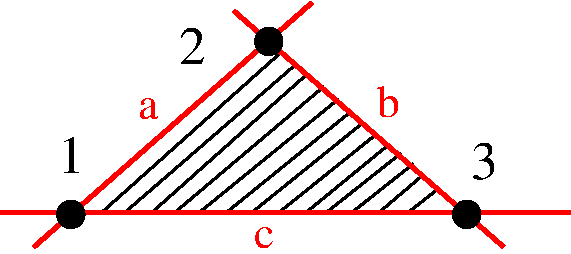
\includegraphics[scale=0.4]{CP2Area2}}}
~\rightarrow~
\begin{array}{l} 
	\mathsf{W}_1=\langle *, \mathsf{Z}_c, \mathsf{Z}_a\rangle \\ 
	\mathsf{W}_2=\langle *, \mathsf{Z}_a, \mathsf{Z}_b\rangle \\ 
	\mathsf{W}_3=\langle *, \mathsf{Z}_b, \mathsf{Z}_c\rangle\,,
	\label{WfromZ}
\end{array}
\end{equation}
\section{Grassmanian}
The Grassmanian $G(k,n)$ is the space of k-planes going through the origin in $n$ dimensions. It can be though of as a generalization of $P^{n-1}$ which is the space of lines going through the origin in $n$-dimensions since $G(1,n)=P^{n-1}$. One can e.g. take $k$ vectors in $n$ dimensions
\begin{figure}
	\centering
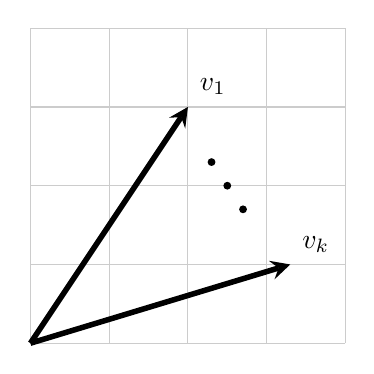
\begin{tikzpicture}
	\draw[thin,gray!40] (0,0) grid (4,4);
	\draw[line width=2pt,black,-stealth](0,0)--(2,3) node[anchor=south west]{$\boldsymbol{v_1}$};
	\node at (2.3,2.3) [circle,fill,inner sep=1pt]{};
	\node at (2.5,2.0) [circle,fill,inner sep=1pt]{};
	\node at (2.7,1.7) [circle,fill,inner sep=1pt]{};
	\draw[line width=2pt,black,-stealth](0,0)--(3.3,1) node[anchor=south west]{$\boldsymbol{v_k}$};
\end{tikzpicture}
\end{figure}
The span of these vectors give me the $k$- plane. If we stack them we get
\begin{equation}
\begin{aligned}
	&~~~~~~~n\\
	k&
\begin{bmatrix}
	~~~~V_1~~~~~\\
	~~~~\vdots ~~~~~\\
	~~~~V_k~~~~~\\
\end{bmatrix}\equiv C_{\alpha a},~~~~~~~~\alpha=1,\dots,k~~~~a=1,\dots,n
\end{aligned}
\end{equation}
These are in general not unique since there is a GL($k$) redundant.
\begin{equation}
C_{\alpha a}\sim L^{\beta}_\alpha C_{\beta a}
\end{equation}
The dimensionality of the Grassmanian is 
\begin{equation}
\dim G(k,n)=\overbrace{k\times n}^{k\times n \text{ matrix}}\underbrace{-k^2}_{GL(k) \text{ red}}
\end{equation}
The redudancy means that we can gaugefix the matrix using a linear transformation by setting any $k\times k$ blok to the identity. This is equivalent to the rescaling of vectors in projective space to $\begin{pmatrix}
1 & v_2 & v_3 & v_4 \cdots
\end{pmatrix}$. Taking e.g. $G(3,5)$, we have six degrees of freedom:
\begin{equation}G(3,5) = 
\left[ \begin{array}{@{}c|c@{}}
	\begin{matrix}
		1 & 0 &  0 \\
		0 & 1 &  0 \\
		0 & 0 &  1 \\
	\end{matrix} 
	& 	\begin{matrix}
		x_4 & x_5  \\
		y_4 & y_5  \\
		z_4 & z_5  \\
	\end{matrix}  \\
\end{array} \right]
\end{equation}
The dimensionality of the Grassmanian are symmetric under $n\leftrightarrow k$. This is because there is a bijection between the Grassmania: $k$ and $n-k$ planes in $n$ dimensions, since these planes are orthogonal. In the case above $C^{\perp}$ is a $2$-plane in 5 dimensions, so
\begin{equation}
	\left[ \begin{array}{@{}c|c@{}}
		\begin{matrix}
			1 & 0 &  0 \\
			0 & 1 &  0 \\
			0 & 0 &  1 \\
		\end{matrix} 
		& 	\begin{matrix}
			x_4 & x_5  \\
			y_4 & y_5  \\
			z_4 & z_5  \\
		\end{matrix}  \\
	\cmidrule[0.4pt]{1-2}
		\begin{matrix}
		-x_4 & -y_4 & -z_4  \\
		-x_5 & -y_5 & -z_5 \\
	\end{matrix} 
	& 	\begin{matrix}
	1 & 0  \\
	0 & 1  \\
\end{matrix} 
	\end{array} \right]
\end{equation}
With the bottom part just being the negative transpose of the $x,y$ and $z$ coordinates in the upper right corner. \\\\
SL$(k)$ invariant are determinants of any $k$ coloumns of the matrix (the minors), labeling these by their indices:
\begin{equation}
\begin{pmatrix}
a_1&a_2&\cdots &a_k
\end{pmatrix}
\end{equation}
\newpage
\section{On-shell diagrams}
\subsection{Using three point on shell functions}
The three-point vertex can be found from the following MHV and $\overline{\text{MHV}}$ diagrams
\begin{figure}[H]\centering\hspace*{3.5cm}
	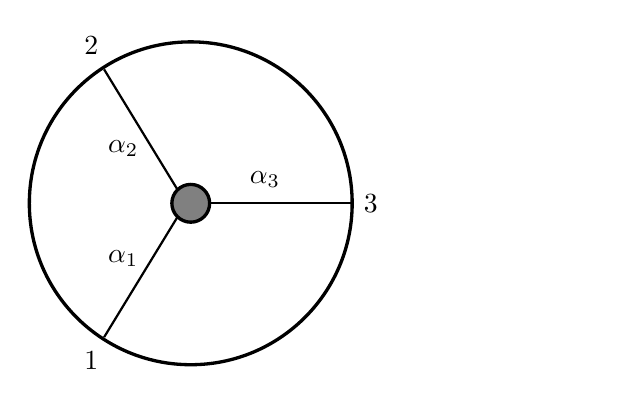
\begin{tikzpicture}
		\begin{scope}[very thick, every node/.style={sloped,allow upside down}]
			\draw[black,fill=gray] (0,0) circle (2.4mm);
			\draw (0,0) circle (20.5mm);
			\draw[thick,black] (-1.1,1.7) -- node {\midarrow} (-0.16,0.16);
			\draw[thick,black] (-1.1,-1.7) -- node {\midarrow} (-0.16,-0.16);
			\draw[thick,black] (0.24,0) -- node {\midarrow} (2.05,0);
			\node[text width=0.5cm] at (-1.1,2.0) {2};
			\node[text width=0.5cm] at (-1.1,-2.0) {1};
			\node[text width=3cm] at (3.7,0) {3};
				\node[text width=0.5cm] at (-0.8,-0.7) {$\alpha_1$};
				\node[text width=0.5cm] at (-0.8,0.7) {$\alpha_2$};
				\node[text width=0.5cm] at (1,0.3) {$\alpha_3$};
		\end{scope}
	\end{tikzpicture}
\end{figure}
\begin{figure}[H]\centering\hspace*{3.5cm}
	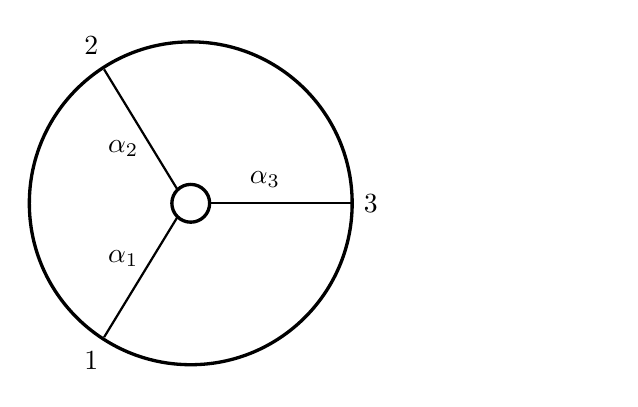
\begin{tikzpicture}
		\begin{scope}[very thick, every node/.style={sloped,allow upside down}]
			\draw[black] (0,0) circle (2.4mm);
			\draw (0,0) circle (20.5mm);
			\draw[thick,black] (-1.1,1.7) -- node {\midarrow} (-0.16,0.16);
			\draw[thick,black] (-1.1,-1.7) -- node {\midarrow} (-0.16,-0.16);
			\draw[thick,black] (0.24,0) -- node {\midarrow} (2.05,0);
			\node[text width=0.5cm] at (-1.1,2.0) {2};
			\node[text width=0.5cm] at (-1.1,-2.0) {1};
			\node[text width=3cm] at (3.7,0) {3};
			\node[text width=0.5cm] at (-0.8,-0.7) {$\alpha_1$};
			\node[text width=0.5cm] at (-0.8,0.7) {$\alpha_2$};
			\node[text width=0.5cm] at (1,0.3) {$\alpha_3$};
		\end{scope}
	\end{tikzpicture}
\end{figure}
These produce the two following $C$ matrices, respectively
\begin{equation}
	\begin{aligned}
		C&=\begin{pmatrix}
			1 & 0 & \alpha_1\alpha_2 \\ 0 & 1 & \alpha_2\alpha_3
		\end{pmatrix}\\
	C&=\begin{pmatrix}
		\alpha_1\alpha_3 \alpha_2\alpha_3 & 1
	\end{pmatrix}
	\end{aligned}
\end{equation}
Note that as opposed to what we will see in the four-point case, here we have no choice in what starting points we take, since e.g. in the MHV ($k=2$) case, we have to pick $1$ and $2$. Because of momentum conservation and little group invariance, the solution of the delta functions in this case leads to 
\begin{equation}
	\begin{aligned}
		A_3^{\text{MHV}}(1,2,3)&=\frac{\delta^{8}\left(\sum_{i=1}^{3}\lambda_i\tilde\eta_i\right)\delta^{4}\left(\sum_{i=1}^{3}\lambda_i\tilde\lambda_i\right)}{\expval{12}\expval{23}\expval{31}}\\
		A_3^{\overline{\text{MHV}}}(1,2,3)&=\frac{\delta^{4}\left([12]\tilde\eta_3+[23]\tilde\eta_1+[31]\tilde\eta_2\right)\delta^{4}\left(\sum_{i=1}^{3}\lambda_i\tilde\lambda_i\right)}{[12][23][31]}\\
	\end{aligned}
\end{equation}
We start by constructing the simplest possible diagram out of two opposite helicity ($k=1$ and $k=2$) amplitudes, see figure below:
\begin{figure}[H]\centering\hspace*{3cm}
	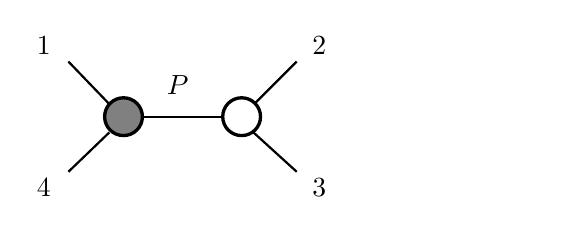
\begin{tikzpicture}
		\begin{scope}[very thick, every node/.style={sloped,allow upside down}]
			\draw (1.5,1.5) circle (2.4mm);
			\draw[black,fill=gray] (0,1.5) circle (2.4mm);
			\draw[thick,black] (0.25,1.5) -- node {\midarrow} (1.25,1.5);
			\node[text width=0.5cm] at (0.8,1.9) {$P$};
			\draw[thick,black] (-0.18,1.3) --  (-0.7,0.8); %4
			\draw[thick,black] (1.67,1.67) --   (2.2,2.2);
			\draw[thick,black] (-0.7,2.2) -- (-0.19,1.67);
			\draw[thick,black] (2.2,0.8) -- (1.65,1.3); %3
			\node[text width=3cm] at (0.4,2.4) {1};
			\node[text width=3cm] at (3.9,2.4) {2};
			\node[text width=3cm] at (3.9,0.6) {3};
			\node[text width=3cm] at (0.4,0.6) {4};
		\end{scope}
	\end{tikzpicture}
\end{figure}
To construct the four-point diagram we then glue the two three-point amplitudes together by integrating over the internal degrees of freedom through
\begin{equation}
	\begin{aligned}
		\prod_{I}\int \dd^4 \tilde \eta_I \int\frac{d^2\lambda_Id^2\tilde\lambda_I}{GL(1)}
	\end{aligned}
\end{equation}
Explicitly we have
\begin{equation}
	\begin{aligned}
		\int \dd \tilde \eta_{P} \int\frac{d^2\lambda_Pd^2\tilde\lambda_P}{GL(1)}&
		\frac{\delta^{8}\left(\lambda_1\tilde\eta_1+\lambda_{4}\tilde\eta_{4}+\lambda_{P}\tilde\eta_{P}\right)\delta^{4}\left(\lambda_{1}\tilde\lambda_{1}+\lambda_{4}\tilde\lambda_{4}+\lambda_{P}\tilde\lambda_{P}\right)}{\expval{14}\expval{4P}\expval{P1}}\\
		\times&\frac{\delta^{4}\left([23]\tilde\eta_{P}+[3P]\tilde\eta_{2}+[P 3]\tilde\eta_{3}\right)\delta^{4}\left(\lambda_{2}\tilde\lambda_{2}+\lambda_{3}\tilde\lambda_{3}-\lambda_{P}\tilde\lambda_{P}
			\right)}{[23][3P][P2]}
	\end{aligned}
\end{equation}
First we solve the delta-function constraint by projecting along $\lambda_1$
\begin{equation}
	\begin{aligned}
		&\lambda_{1}\tilde\lambda_{1}+\lambda_{4}\tilde\lambda_{4}+\lambda_{P}\tilde\lambda_{P}=0\\
		\Rightarrow& \tilde\lambda_{P}=\frac{\expval{41}}{\expval{1P}}\tilde\lambda_4
	\end{aligned}
\end{equation}
Similarly we use the other delta-function and project using $\tilde \lambda_3$
\begin{equation}
	\begin{aligned}
		&\lambda_{2}\tilde\lambda_{2}+\lambda_{3}\tilde\lambda_{3}-\lambda_{P}\tilde\lambda_{P}=0\\
		\Rightarrow& 
		\lambda_{P}=\frac{[23]}{[P3]}\lambda_2
	\end{aligned}
\end{equation}
combining these we obtain
\begin{equation}
	\begin{aligned}
		\tilde\lambda_P \lambda_P=\lambda_2 \tilde\lambda_4 \frac{\expval{41}[23]}{\expval{1P}[P3]}&=\lambda_2 \tilde\lambda_4 \frac{[23]}{[43]}\\
		&=\lambda_2 \tilde\lambda_4 \frac{\expval{41}}{\expval{12}}
 	\end{aligned}
\end{equation}
where we have used $P=-1-4=2+3$ in the last two equalities. Solving this collapses the momentum conservation delta function as well as giving a Jacobian factor of $\frac{1}{\expval{23}[32]}$
\begin{equation} \label{eq:sol3}
	\begin{aligned}
		\lambda_P&=\lambda_2\\
		\tilde \lambda_P&=\lambda_4 \frac{\expval{41}}{\expval{12}}=\tilde\lambda_4 \frac{[23]}{[43]}
	\end{aligned}
\end{equation}
We then use these in one of the grassmann delta-functions
\begin{equation}
	\begin{aligned}
		\tilde\eta_{P}&=\frac{-[3P]\tilde\eta_{2}-[P 2]\tilde\eta_{3}}{[23]}\\
		&=-\frac{1}{[23]}\times \frac{[34][23]}{[43]} \times\tilde \eta_2-\frac{1}{[23]}\times \frac{[42]\expval{41}}{\expval{12}} \times\tilde \eta_3\\
		&=\tilde \eta_2+ \frac{\expval{13}}{\expval{12}} \times\tilde \eta_3\\
	\end{aligned}
\end{equation}
This can be obtained from contracting
\begin{equation}
	\begin{aligned}
\lambda_P\tilde\eta_{P}	&=\lambda_2\tilde \eta_2+ \lambda_3 \tilde \eta_3\\	
	\end{aligned}
\end{equation}
 with $\lambda_1$, since $\lambda_P=\lambda_2$. Using this in the other grassmann  delta function we get $[23]^4\delta^8(\sum_i\lambda_i\tilde\eta_i)$. Finally we take the solutions \eqref{eq:sol3} and insert them into the bosonic delta-function
 \begin{equation}
 	\begin{aligned}
 		0&=\lambda_1\tilde\lambda_1+\lambda_4\tilde\lambda_4+\lambda_P\tilde\lambda_P\\
 		&=\lambda_1\tilde\lambda_1+\lambda_4\tilde\lambda_4+\lambda_2\tilde\lambda_4  \frac{[23]}{[43]}\\
 		&=\lambda_1\tilde\lambda_1+\tilde\lambda_4 \left(\lambda_4+\lambda_2  \frac{[23]}{[43]}\right)
 		\\
 		&=\lambda_1\tilde\lambda_1+\tilde\lambda_4 \left(  \frac{\lambda_4[43]+\lambda_2[23]}{[43]}\right)
 		\\
 		&=\lambda_1\tilde\lambda_1+\tilde\lambda_4 \left(  \frac{(2+4)|3]}{[43]}\right)
 		\\
 		&=\lambda_1\tilde\lambda_1-\tilde\lambda_4 \left(  \frac{\lambda_1[13]}{[43]}\right)
 		\\
 		&=\lambda_1 \left(\tilde\lambda_1 +\tilde\lambda_4 \frac{[13]}{[34]}\right)
 			\\
 		&=\lambda_1 \left( \frac{\tilde\lambda_1[34]+\tilde\lambda_4[13]}{[34]}\right)
 			\\
 		&=\lambda_1 \tilde\lambda_3 \frac{[14]}{[34]}
 	\end{aligned}
 \end{equation}
Since $\lambda_1\neq0,$ and $\tilde\lambda_3\neq0$ this leads to $[14]=0$ which in turn gives us
\begin{equation}
	\begin{aligned}
		(p_1+p_4)^2=\expval{14}[41]=0
	\end{aligned}
\end{equation}
Now we only need the kinematic part of the integrand. Including the Jacobians and using $\expval{1P}[P3]=\expval{12}[23]$ and $\expval{4P}[P2]=\expval{43}[32]$ we obtain
\begin{equation}
	\begin{aligned}
		\frac{1}{\expval{14}\expval{4P}\expval{P1}}\times\frac{1}{[23][3P][P2]}\times \frac{[23]^4}{\expval{23}[23]}&=\frac{1}{\expval{12}\expval{23}\expval{34}\expval{41}}\\
	\end{aligned}
\end{equation}
Such that we in total have the amplitude
\begin{equation}
	\begin{aligned}
		\frac{\delta^{8}\left(\mathcal{Q}\right)\delta^{4}\left(P\right)}{\expval{12}\expval{23}\expval{34}\expval{41}}\delta((p_1+p_4)^2)
	\end{aligned}
\end{equation}
Continuing this approach, we then look at the four-point on-shell diagram. We bridge together two of the diagrams just obtained
\begin{figure}[H]\centering\hspace*{3cm}
	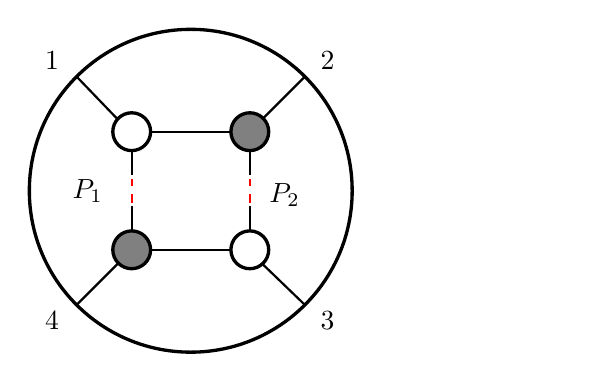
\begin{tikzpicture}
		\begin{scope}[very thick, every node/.style={sloped,allow upside down}]
			\draw[black,fill=gray] (0,0) circle (2.4mm);
			\draw (1.5,0) circle (2.4mm);
			\draw[black,fill=gray] (1.5,1.5) circle (2.4mm);
			\draw (0,1.5) circle (2.4mm);
			\draw[thick,black] (1.25,0) --  (0.25,0);
			\draw[thick,black] (0.25,1.5) -- (1.25,1.5);
			\draw[thick,black]  (0,0.95) -- (0,1.25);
			\draw[thick,black]  (0,0.25) -- (0,0.55);
			\draw[thick,red,dashed] (0,0.6) -- (0,0.9) ;
			\node[text width=0.5cm] at (-0.5,0.75) {$P_1$};
			\draw[thick,black] (1.5,0.95) -- (1.5,1.25) ;
			\draw[thick,black] (1.5,0.25) -- (1.5,0.55) ;
			\draw[thick,red,dashed] (1.5,0.6) -- (1.5,0.9) ;
			\node[text width=0.5cm] at (2,0.7) {$P_2$};
			\draw[thick,black] (-0.18,-0.18) --  (-0.7,-0.7);
			\draw[thick,black] (1.67,1.67) --   (2.2,2.2);
			\draw[thick,black] (-0.7,2.2) -- (-0.19,1.67);
			\draw[thick,black] (2.2,-0.7) -- (1.65,-0.17);
			\draw (0.75,0.75) circle (20.5mm);
			\node[text width=3cm] at (0.4,2.4) {1};
			\node[text width=3cm] at (3.9,2.4) {2};
			\node[text width=3cm] at (3.9,-0.9) {3};
			\node[text width=3cm] at (0.4,-0.9) {4};
		\end{scope}
	\end{tikzpicture}
\end{figure}
We have the following integral
\begin{equation}
	\begin{aligned}
		\int \dd \eta_{P_1} \dd \eta_{P_2}\int&\frac{d^2\lambda_{P_1}d^2\tilde\lambda_{P_1}d^2\lambda_{P_2}d^2\tilde\lambda_{P_2}}{\text{Vol}(GL(1))\times\text{Vol}(GL(1))}\times \Omega (1,2,P_2,P_1)\times \Omega (P_1,P_2,3,4)
	\end{aligned}
\end{equation}
\begin{equation}
	\begin{aligned}
		&\int \dd \eta_{P_1} \dd \eta_{P_2}\int\frac{d^2\lambda_{P_1}d^2\tilde\lambda_{P_1}d^2\lambda_{P_2}d^2\tilde\lambda_{P_2}}{\text{Vol}(GL(1))\times\text{Vol}(GL(1))}\\&\times 	\frac{\delta^{8}\left(\lambda_{1}\tilde \eta_{1}+\lambda_{2}\tilde \eta_{2}+\lambda_{P_1}\tilde \eta_{P_1}+\lambda_{P_2}\tilde \eta_{P_2}\right)\delta^{4}\left(\lambda_{1}\tilde\lambda_{1}+\lambda_{2}\tilde\lambda_{2}+\lambda_{P_2}\tilde\lambda_{P_2}-\lambda_{P_1}\tilde\lambda_{P_1}\right)}{\expval{12}\expval{2P_2}\expval{P_2P_1}\expval{P_11}}\delta(\expval{1P_1}[P_1 1])
		\\&\times 	\frac{\delta^{8}\left(\lambda_{3}\tilde \eta_{3}+\lambda_{4}\tilde \eta_{4}+\lambda_{P_1}\tilde \eta_{P_1}+\lambda_{P_2}\tilde \eta_{P_2}\right)\delta^{4}\left(\lambda_{3}\tilde\lambda_{3}+\lambda_{4}\tilde\lambda_{4}-\lambda_{P_2}\tilde\lambda_{P_2}+\lambda_{P_1}\tilde\lambda_{P_1}\right)}{\expval{34}\expval{4P_1}\expval{P_1P_
			2}\expval{P_23}}\delta(\expval{4P_1}[P_1 4])
	\end{aligned}
\end{equation}
We use the bosonic delta-function to solve for $\lambda_{P_i}$ and $\tilde\lambda_{P_i}$ while assuming $[P_1 1]=[P_1 4]=0$ so that the delta-function forcing the amplitude on the s-channel simplifies, while keeping the integrand from blowing up. Contracting with $\lambda_1$ and $\lambda_4$
\begin{equation}
	\begin{aligned}
		\expval{12}\tilde\lambda_{2}+\expval{1P_2}\tilde\lambda_{P_2}-\expval{1P_1}\tilde\lambda_{P_1}=0\\
		\expval{43}\tilde\lambda_{3}-\expval{4P_2}\tilde\lambda_{P_2}+\expval{4P_1}\tilde\lambda_{P_1}=0
	\end{aligned}
\end{equation}
Solving for the $\lambda$'s we find
\begin{equation}
	\begin{aligned}
		\tilde \lambda_{P_1}&=\frac{\tilde{\lambda}_3
		\expval{1P_2}\expval{34}
		-
		\tilde{\lambda}_2
		\expval{12}\expval{4P_2}
	}{\expval{1P_2}\expval{4P_1}
	-
	\expval{1P_1}\expval{4P_2}}
=\frac{\tilde{\lambda}_3
	\expval{1P_2}\expval{34}
	-
	\tilde{\lambda}_2
	\expval{12}\expval{4P_2}
}{\expval{14}\expval{P_2P_1}}
\\
		\tilde \lambda_{P_2}&=\frac{\tilde{\lambda}_3
	\expval{1P_1}\expval{34}
	-
	\tilde{\lambda}_2
	\expval{12}\expval{4P_1}
}{\expval{1P_2}\expval{4P_1}
	-
	\expval{1P_1}\expval{4P_2}}=\frac{\tilde{\lambda}_3
	\expval{1P_1}\expval{34}
	-
	\tilde{\lambda}_2
	\expval{12}\expval{4P_1}
}{\expval{14}\expval{P_2P_1}}\\
	\end{aligned}
\end{equation}
Similar we can contract with $ \tilde \lambda_2$ and $\tilde \lambda_3$
\begin{equation}
	\begin{aligned}
		\lambda_1[12]+\lambda_{P_2}[P_2 2]-\lambda_{P_1}[P_1 2]&=0\\
		\lambda_3[34]-\lambda_{P_2}[P_2 4]+\lambda_{P_1}[P_1 4]&=0\\
	\end{aligned}
\end{equation}
to obtain
\begin{equation}
	\begin{aligned}
		\lambda_{P_1}&=\frac{\lambda_3[2P_2][34]+\lambda_2[4P_2][12]}{[2P_2][4P_1]-[2P_1][4P_2]}=\frac{\lambda_3[2P_2][34]+\lambda_2[4P_2][12]}{[24][P_2P_1]}\\
		\lambda_{P_2}&=\frac{\lambda_3[2P_1][34]+\lambda_2[4P_1][12]}{[2P_2][4P_1]-[2P_1][4P_2]}=\frac{\lambda_3[2P_2][34]+\lambda_2[4P_2][12]}{[24][P_2P_1]}
	\end{aligned}
\end{equation}
%%%%%%%%%%%%%%%%%%%%%%%%%%%%%%%%%%%%%%%%%%%%%%%%%%%%%%%%%%%%%%%%%%%%%%%%%%%%%%%%%%%%%%%%%%%%%%%%%%%%%%%%%%%%%%%%%%%%%%%%%%%%%%%%%%%%%%%%%%%%%%%%%%%%%%%%%%%%%%%%%%%%%%%%%%%%%%%%%%%%%%%%%%%%%%%%%%%%%%%%%%%%%%%%%%%%%%%%%%%%%%%%%%%%%%%%%%%%%%%%%%%%%%%%%%%%%%%%

The grassmann integral is easily seen to just produce $\delta^8(\sum_i\lambda_i\tilde \eta_i)$ while the bosonic delta functions collapse the spinor products into a single delta-function $\delta^4(\sum_i\lambda_i\tilde \lambda_i)$. Finally 
%%%%%%%%%%%%%%%%%%%%%%%%%%%%%%%%%%%%%%%%%%%%%%%%%%%%%%%%%%%%%%%%%%%%%%%%%%%%%%%%%%%%%%%
\subsection{Four-point directly from C(2,4) matrix}
The calculation this C-matrix can be performed either using face or edge variables. We are going to do both for good measure.
The four-point diagram with face-variables looks like this
%%%%%%%%%%%%%%%%%%%%%%%%%%%%%%%%%%%%%%%%%%%%%%%%%%%%%%%%%%%%%%%%%%%%%%%%
\begin{figure}[H]\centering \hspace*{3cm}
	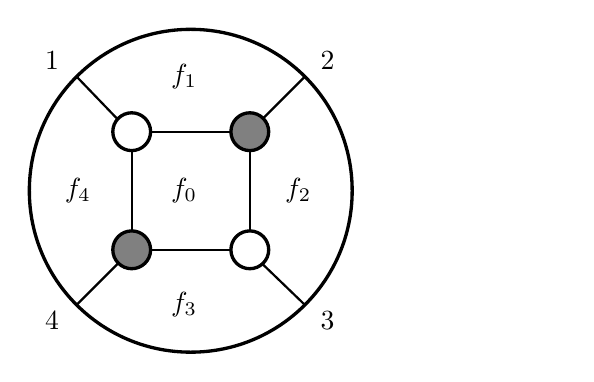
\begin{tikzpicture}
		\begin{scope}[very thick, every node/.style={sloped,allow upside down}]
			\draw[black,fill=gray] (0,0) circle (2.4mm);
			\draw (1.5,0) circle (2.4mm);
			\draw[black,fill=gray] (1.5,1.5) circle (2.4mm);
			\draw (0,1.5) circle (2.4mm);
			\draw[thick,black] (1.25,0) -- node {\midarrow} (0.25,0);
			\node[text width=0.5cm] at (0.75,-0.7) {$f_3$};
			\draw[thick,black] (0.25,1.5) -- node {\midarrow} (1.25,1.5);
			\node[text width=0.5cm] at (0.75,2.2) {$f_1$};
			\draw[thick,black] (0,1.25) -- node {\midarrow} (0,0.25);
			\node[text width=0.5cm] at (-0.6,0.75) {$f_4$};
			\draw[thick,black] (1.5,1.25) -- node {\midarrow} (1.5,0.25);
			\node[text width=0.5cm] at (2.2,0.75) {$f_2$};
			\node[text width=0.5cm] at (0.75,0.75) {$f_0$};
			\draw[thick,black] (-0.18,-0.18) -- node {\midarrow} (-0.7,-0.7);
			\draw[thick,black] (2.2,2.2) --  node {\midarrow}  (1.67,1.67) ;
			\draw[thick,black] (-0.7,2.2) -- node {\midarrow} (-0.19,1.67);
			\draw[thick,black] (1.65,-0.17) -- node {\midarrow} (2.2,-0.7);
			\draw (0.75,0.75) circle (20.5mm);
			\node[text width=3cm] at (0.4,2.4) {1};
			\node[text width=3cm] at (3.9,2.4) {2};
			\node[text width=3cm] at (3.9,-0.9) {3};
			\node[text width=3cm] at (0.4,-0.9) {4};
		\end{scope}
	\end{tikzpicture}
\end{figure}
While the
\begin{equation}
	\begin{aligned}
		C_{ab}=-\sum_{\Gamma(a\to b)}\prod_j\left(-f_j\right),~~~~~~\text{ on the right} 
	\end{aligned}
\end{equation}
with the constraint
\begin{equation}
	\begin{aligned} \label{eq:prodf}
		\prod_j f_j=-1
	\end{aligned}
\end{equation}
%%%%%%%%%%%%%%%%%%%%%%%%%%%%%%%%%%%%%%%%%%%%%%%%%%%%%%%%%%%%%%%%%%%%%%%%%%%%%%%%%%%%%%%%%%%%%%%%%%%%%%%%%%%%%%%%%%%%%%%%%%%%%%%
\begin{equation}
	\begin{aligned}
		C=
		\begin{pmatrix}
			1 & 0 & f_0f_3f_4 & f_4(1-f_0)\\
			0 & 1 & -f_0f_1f_3f_4&f_0f_1f_4
		\end{pmatrix}
	\end{aligned}
\end{equation}
Note that $f_2$ doesn't show up, which means that according to \eqref{eq:prodf} we can take the remaining $f$'s as independent.

Positivity (all minors are positive) then demands that
\begin{equation}
	\begin{aligned}
		f_0<0,~~~~f_1>0,~~~~f_2<0,~~~~f_3<0,~~~~
	\end{aligned}
\end{equation}
While the perpendicular C-matrix satisfying $C\cdot C^\perp=0$ is easily obtained
\begin{equation}
	\begin{aligned}
		C^\perp=
		\begin{pmatrix}
		 -f_0f_3f_4 &f_0f_1f_3f_4 & 1 & 0\\
		-f_4(1-f_0) &-f_0f_1f_4 & 0 & 1
		\end{pmatrix}
	\end{aligned}
\end{equation}
we can then find the form through
\begin{equation}
	\begin{aligned}
		\dd \Omega =\frac{\dd f_0}{f_0}\frac{\dd f_1}{f_1}\frac{\dd f_3}{f_3}\frac{\dd f_4}{f_4}\delta(C\cdot \tilde \lambda) \delta(C^\perp\cdot \lambda)\delta(C\cdot \tilde \eta)
	\end{aligned}
\end{equation}
First let us look at the delta-functions, such that we can specify the face-variables in terms of the spinor products. We start by looking at $C\cdot C^\perp=0$, from which we can two equations
\begin{equation}
	\begin{aligned}
		C^\perp\cdot \lambda=0\Rightarrow\begin{cases}
			-\lambda_1f_0f_3f_4+\lambda_2 f_0f_1f_3f_4+ \lambda_3&=0\\
			-\lambda_1f_4(1-f_0)-\lambda_2f_0f_1f_4+ \lambda_4&=0
		\end{cases}
	\end{aligned}
\end{equation}
By multiplying the first equation by $\tilde \lambda_2$ one obtains $f_0f_3f_4=-\frac{\expval{23}}{\expval{12}}$. Similarly multiplying the second equation by $\tilde \lambda_1$ we get $f_0f_1f_4= \frac{\expval{14}}{\expval{12}}$. Combining these two,
\begin{equation}
	\begin{aligned}
		f_1=-\frac{\expval{14}}{\expval{23}}f_3
	\end{aligned}
\end{equation}
Then multiplying the first equation by $\tilde\lambda_1$ we have $f_0f_1f_3f_4=-\frac{\expval{13}}{\expval{12}}$ together with the previous result, this leads to
\begin{equation}
	\begin{aligned}
		f_3 =-\frac{\expval{13}}{\expval{14}} ~~~~~\text{and }~~~~~f_1 =\frac{\expval{13}}{\expval{23}} 
	\end{aligned}
\end{equation}
The other equations are solved similarly and we obtain
\begin{equation}
	\begin{aligned}
		f_0=&-\frac{\expval{14}\expval{23}}{\expval{12}\expval{34}}\\
		f_4=&-\frac{\expval{34}}{\expval{13}} 
	\end{aligned}
\end{equation}
%%%%%%%%%%%%%%%%%%%%%%%%%%%%%%%%%%%%%%%%%%%%%%%%%%%%%%%%%%%%%%%%%%%%%%%%
Let us now evaluate the two remaining delta-functions. From $C\cdot \tilde \lambda$ we get two equations. 
\begin{equation}
	\begin{aligned}
		0=\tilde\lambda_1+f_0f_3f_4 \tilde\lambda_3+f_4(1-f_0)\tilde\lambda_4=\tilde\lambda_1+\frac{\expval{32}}{\expval{12}} \tilde\lambda_3+\frac{\expval{42}}{\expval{12}} \tilde\lambda_4
	\end{aligned}
\end{equation}
and
\begin{equation}
	\begin{aligned}
		0=\tilde\lambda_2+\frac{\expval{13}}{\expval{12}} \tilde\lambda_3+\frac{\expval{14}}{\expval{12}} \tilde\lambda_4
	\end{aligned}
\end{equation}
where we have used a Schouten identity for the coefficient of $\tilde\lambda_4$
\begin{equation}
	\begin{aligned}
		\expval{41}\expval{23}+\expval{12}\expval{34}=\expval{13}\expval{24}
	\end{aligned}
\end{equation}
We see that these equations can all be obtained from a momentum conservation delta-function by contracting it with $\lambda_1$ and $\lambda_2$
\begin{equation}
\begin{aligned}
	\delta^{4}(\lambda_1\tilde\lambda_1+\lambda_2\tilde\lambda_2+\lambda_3\tilde\lambda_3+\lambda_4\tilde\lambda_4)\equiv \delta^{4}\left(P\right)
\end{aligned}
\end{equation}
For the last delta-function we get the exact same thing except for replacing $\tilde \lambda_i\to \tilde \eta_i$
\begin{equation}
\begin{aligned}
	\delta^{8}(\lambda_1\tilde\eta_1+\lambda_2\tilde\eta_2+\lambda_3\tilde\eta_3+\lambda_4\tilde\eta_4)\equiv \delta^{8}\left(\mathcal{Q}\right)
\end{aligned}
\end{equation}
Note that we get an extra factor of $\frac{1}{\expval{12}^4}$ from re-writing the delta-functions by projecting along $\lambda_1$ and $\lambda_2$. Finally we get a Jacobian.
\begin{equation}
	\begin{aligned}
		J=\left|J_{ij}\right|=f_0^2f_1f_3f_4^3=\frac{\expval{23}\expval{34}\expval{41}}{\expval{12}^2\expval{13}}
	\end{aligned}
\end{equation}
where
\begin{equation}
	\begin{aligned}
		J_{ij}=\pdv{E_i}{f_j}=\begin{pmatrix}
			f_3f_3 & 0 & f_0f_3 & f_0f_4\\
			f_1f_3f_4 &f_0f_3f_4 &f_0f_1f_4 & f_0f_1f_3\\
			f_4 & 0 & 0 & 1-f_0\\
			f_1f_4 & f_0f_4 & 0 & f_0f_1
		\end{pmatrix}
	\end{aligned}
\end{equation}
and 
\begin{equation}
	\begin{aligned}
		E_1=f_0f_3f_4,~~~~E_2=f_0f_1f_3f_4,~~~~E_3=f_4(1-f_0),~~~~E_4=f_0f_1f_3
	\end{aligned}
\end{equation}
Now using
\begin{equation}
	\begin{aligned}
		f_0f_1f_3f_4=\frac{\expval{13}}{\expval{12}}
	\end{aligned}
\end{equation}
We can put it all together to obtain the form
\begin{equation}
	\begin{aligned}
		\dd \Omega =\frac{\expval{12}}{\expval{13}}\times \frac{\expval{12}^2\expval{13}}{
			\expval{23}\expval{34}\expval{41}}\times \frac{1}{\expval{12}^4}\times \delta^4(P)\delta^8(\mathcal{Q})=\frac{\delta^{8}\left(\mathcal{Q}\right)\delta^{4}\left(P\right)}{\expval{12}\expval{23}\expval{34}\expval{41}}
	\end{aligned}
\end{equation}
%%%%%%%%%%%%%%%%%%%%%%%%%%%%%%%%%%%%%%%%%%%%%%%%%%%%%%%%%%%%%%%%%%%%%%%%

For the edge-variable case let us try a different orientation
\begin{figure}[H]\centering\hspace*{3cm}
	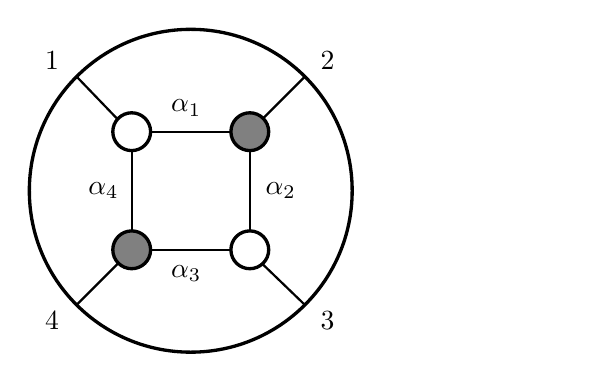
\begin{tikzpicture}
		\begin{scope}[very thick, every node/.style={sloped,allow upside down}]
			\draw[black,fill=gray] (0,0) circle (2.4mm);
			\draw (1.5,0) circle (2.4mm);
			\draw[black,fill=gray] (1.5,1.5) circle (2.4mm);
			\draw (0,1.5) circle (2.4mm);
			\draw[thick,black] (1.25,0) -- node {\midarrow} (0.25,0);
			\node[text width=0.5cm] at (0.75,-0.3) {$\alpha_3$};
			\draw[thick,black] (0.25,1.5) -- node {\midarrow} (1.25,1.5);
			\node[text width=0.5cm] at (0.75,1.8) {$\alpha_1$};
			\draw[thick,black] (0,1.25) -- node {\midarrow} (0,0.25);
			\node[text width=0.5cm] at (-0.3,0.75) {$\alpha_4$};
			\draw[thick,black] (1.5,0.25) -- node {\midarrow} (1.5,1.25);
			\node[text width=0.5cm] at (1.95,0.75) {$\alpha_2$};
			\draw[thick,black] (-0.18,-0.18) -- node {\midarrow} (-0.7,-0.7);
			\draw[thick,black] (1.67,1.67) --  node {\midarrow} (2.2,2.2);
			\draw[thick,black] (-0.7,2.2) -- node {\midarrow} (-0.19,1.67);
			\draw[thick,black] (2.2,-0.7) -- node {\midarrow} (1.65,-0.17);
			\draw (0.75,0.75) circle (20.5mm);
			\node[text width=3cm] at (0.4,2.4) {1};
			\node[text width=3cm] at (3.9,2.4) {2};
			\node[text width=3cm] at (3.9,-0.9) {3};
			\node[text width=3cm] at (0.4,-0.9) {4};
		\end{scope}
	\end{tikzpicture}
\end{figure}
Here the $C$-matrix is now giving by
\begin{equation}
	\begin{aligned}
		C_{ab}=\sum_{\Gamma(a\to b)}\prod_j\alpha_j
	\end{aligned}
\end{equation}
%%%%%%%%%%%%%%%%%%%%%%%%%%%%%%%%%%%%%%%%%%%%%%%%%%
SO we get the following
\begin{equation}
	\begin{aligned}
		C=
		\begin{pmatrix}
			1  & \alpha_1 & 0 & \alpha_4\\
			0 &\alpha_2 &1 & \alpha_3
		\end{pmatrix}
	\end{aligned}
\end{equation}
With the inverse
%%%%%%%%%%%%%%%%%%%%%%%%%%%%%%%%%%%%%%%%%%%%%%%%%%%%%%%
\begin{equation}
	\begin{aligned}
		C^\perp=
		\begin{pmatrix}
			-\alpha_1  & 1 & -\alpha_2 & 0\\
			-\alpha_4 & 0 &-\alpha_3 & 1
		\end{pmatrix}
	\end{aligned}
\end{equation}
%%%%%%%%%%%%%%%%%%%%%%%%%%%%%%%%%%%%%%%%%%%%%%%%%%%%%%%%
\begin{equation}
	\begin{aligned}
		C^\perp\cdot \lambda=0\Rightarrow\begin{cases}
			-\alpha_1\lambda_1+\lambda_2-\alpha_3\lambda_3&=0\\
			-\alpha_4\lambda_1-\alpha_2\lambda_3+\lambda_4&=0
		\end{cases}
	\end{aligned}
\end{equation}
turns into
\begin{equation}
	\begin{aligned}
		\expval{21} -\alpha_2 \expval{31}&=0\Rightarrow\alpha_2=\frac{\expval{12}}{\expval{13}}\\
		\alpha_1\expval{12} -\alpha_3\expval{23}&=0 \Rightarrow\alpha_1=\alpha_2\frac{\expval{23}}{\expval{12}}=\frac{\expval{23}}{\expval{13}}
	\end{aligned}
\end{equation}
Similarly we find
\begin{equation}
	\begin{aligned}
		\alpha_3=\frac{\expval{14}}{\expval{13}},~~~~~~~~\alpha_4=\frac{\expval{43}}{\expval{13}}
	\end{aligned}
\end{equation}
For the other delta functions $C\cdot \tilde\lambda$ gives us two equations. The first one is
\begin{equation}
	\begin{aligned}
		0&=\tilde\lambda_1+\alpha_2\tilde\lambda_2+\alpha_4\tilde\lambda_4=\tilde\lambda_1+\frac{\expval{23}}{\expval{13}}\tilde\lambda_2+\frac{\expval{43}}{\expval{13}}\tilde\lambda_4\\
		\Rightarrow 0&=\expval{13}\tilde\lambda_1+\expval{23}\tilde\lambda_2+\expval{43}\tilde\lambda_4
	\end{aligned}
\end{equation}
While the second one is found similarly
\begin{equation}
	\begin{aligned}
		0=\expval{21}\tilde\lambda_2+\expval{31}\tilde\lambda_2+\expval{41}\tilde\lambda_4
	\end{aligned}
\end{equation}
We see that the two equations can be obtained from a single momentum conservation equation by contracting with $\lambda_3$ and $\lambda_1$ respectively. I.e. we have
\begin{equation}
	\begin{aligned}
		\delta^{4}(\lambda_1\tilde\lambda_1+\lambda_2\tilde\lambda_2+\lambda_3\tilde\lambda_3+\lambda_4\tilde\lambda_4)\equiv \delta^{4}\left(P\right)
	\end{aligned}
\end{equation}
For the last delta-function we get the exact same thing except for replacing $\tilde \lambda_i\to \tilde \eta_i$
\begin{equation}
	\begin{aligned}
		\delta^{8}(\lambda_1\tilde\eta_1+\lambda_2\tilde\eta_2+\lambda_3\tilde\eta_3+\lambda_4\tilde\eta_4)\equiv \delta^{8}\left(\mathcal{Q}\right)
	\end{aligned}
\end{equation}
Note that we get an extra factor of $\frac{1}{\expval{13}^4}$ from re-writing the delta-functions in by projecting along $\lambda_1$ and $\lambda_3$.
 Finally we have
\begin{equation}
	\begin{aligned}
		\frac{1}{\alpha_1 \alpha_2 \alpha_3 \alpha_4}=\frac{\expval{13}^4}{\expval{12}\expval{23}\expval{34}\expval{41}}
	\end{aligned}
\end{equation}
We can now calculate the form
\begin{equation}
	\begin{aligned}
		\dd \Omega =
		\frac{\delta^{8}\left(\mathcal{Q}\right)\delta^{4}\left(P\right)}{\expval{12}\expval{23}\expval{34}\expval{41}}
	\end{aligned}
\end{equation}
\subsection{Five point}
\begin{figure}[H]\centering\hspace*{3cm}
	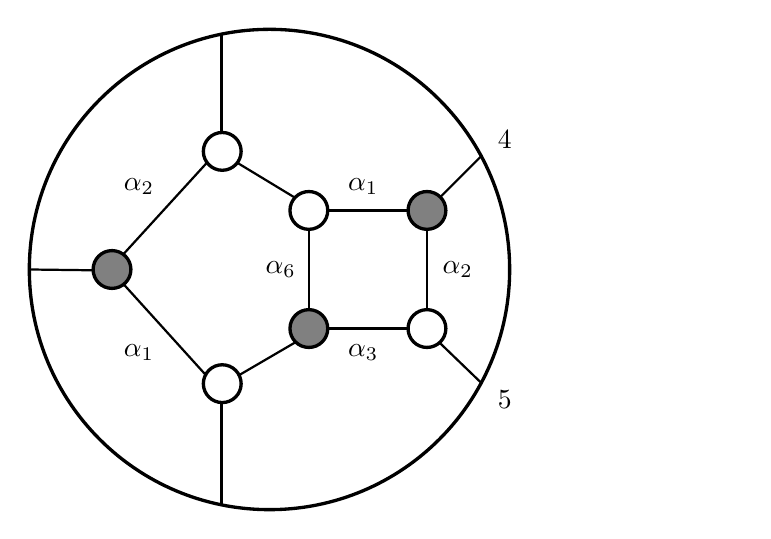
\begin{tikzpicture}
		\begin{scope}[very thick, every node/.style={sloped,allow upside down}]
			\draw[black,fill=gray] (0,0) circle (2.4mm);
			\draw (1.5,0) circle (2.4mm);
			\draw[black,fill=gray] (1.5,1.5) circle (2.4mm);
			\draw (0,1.5) circle (2.4mm);
			\draw (-1.1,2.25) circle (2.4mm);
			\draw (-1.1,-0.7) circle (2.4mm);
			\draw (-2.5,0.75)[black,fill=gray]  circle (2.4mm);
			\draw[thick,black] (1.25,0) -- node {\midarrow} (0.25,0);
			\node[text width=0.5cm] at (0.75,-0.3) {$\alpha_3$};
			\draw[thick,black] (1.25,1.5)  -- node {\midarrow}  (0.25,1.5);
			\node[text width=0.5cm] at (0.75,1.8) {$\alpha_1$};
			\draw[thick,black] (0,1.25) -- node {\midarrow} (0,0.25);
			\node[text width=0.5cm] at (-0.3,0.75) {$\alpha_6$};
			\draw[thick,black] (1.5,0.25) -- node {\midarrow} (1.5,1.25);
			\node[text width=0.5cm] at (1.95,0.75) {$\alpha_2$};
			\draw[thick,black] (1.5,0.25) -- node {\midarrow} (1.5,1.25);
			\draw[thick,black] (-1.3,-0.6) -- node {\midarrow} (-2.35,0.56);
			\node[text width=0.5cm] at (-2.1,-0.3) {$\alpha_1$};
			\draw[thick,black] (-1.3,2.1) -- node {\midarrow} (-2.35,0.95);
			\node[text width=0.5cm] at (-2.1,1.8) {$\alpha_2$};
			%			
			\draw[thick,black] (-0.18,-0.18) -- node {\midarrow} (-0.9,-0.6);
			\draw[thick,black] (-3.55,0.75) -- node {\midarrow} (-2.75,0.74);
			\draw[thick,black] (1.67,1.67) --  node {\midarrow} (2.2,2.2);
			\draw[thick,black] (-0.9,2.1) -- node {\midarrow} (-0.19,1.67);
			\draw[thick,black] (2.2,-0.7) -- node {\midarrow} (1.65,-0.17);
			\draw[thick,black] (-1.11,-2.25) -- node {\midarrow} (-1.11,-0.95);
			\draw[thick,black] (-1.11,3.75) -- node {\midarrow} (-1.11,2.5);
			\draw (-0.5,0.75) circle (30.5mm);
			%\node[text width=3cm] at (0.4,2.4) {1};
			\node[text width=3cm] at (3.9,2.4) {4};
			\node[text width=3cm] at (3.9,-0.9) {5};
			%\node[text width=3cm] at (0.4,-0.9) {4};
		\end{scope}
	\end{tikzpicture}
\end{figure}
Each vertex can fix one edge-variable, however you cannot do it in such a way that all variables in a vertex is fixed.
The $C$ matrix is
\begin{equation}
	\begin{aligned}
		C=\begin{pmatrix}
			1 & \alpha_1+\alpha_2\alpha_6 & \alpha_6 & \alpha_3\alpha_6 & 0\\
			0 & \alpha_5 \alpha_6 \alpha_2 & \alpha_5 \alpha_6 & \alpha_4+\alpha_3\alpha_5\alpha_6 & 1
		\end{pmatrix}
	\end{aligned}
\end{equation}
with the inverse being
\begin{equation}
	\begin{aligned}
		C^\perp =\begin{pmatrix}
			-(\alpha_1+\alpha_2\alpha_6) & 1 & 0 & 0 & -\alpha_5 \alpha_6 \alpha_2\\
			-\alpha_6 & 0 & 1 & 0 & -\alpha_5 \alpha_6 \\
			-\alpha_3 \alpha_6 & 0 & 0 & 1 & -(\alpha_4+\alpha_3\alpha_5\alpha_6)
		\end{pmatrix}
	\end{aligned}
\end{equation}
The amplitude is found through
\begin{equation}
	\begin{aligned}
		\dd \Omega =\frac{\dd \alpha_1}{\alpha_1}\frac{\dd \alpha_2}{\alpha_2}\frac{\dd \alpha_3}{\alpha_3}\frac{\dd \alpha_4}{\alpha_4}\frac{\dd \alpha_5}{\alpha_5}\frac{\dd \alpha_6}{\alpha_6}\delta^{2\times 2}(C\cdot \tilde \lambda) \delta^{2\times 3}(C^\perp\cdot \lambda)\delta^{4\times 2}(C\cdot \tilde \eta)
	\end{aligned}
\end{equation}
Using the delta-function $\delta^{2\times 3}(C^\perp\cdot \lambda)$ to solve for the $\alpha$'s we obtain after contracting with $\lambda_1$, $\lambda_3$, and $\lambda_5$
\begin{equation}
	\begin{aligned}
		\alpha_1=\frac{\expval{23}}{\expval{13}},~~~~
		\alpha_2=\frac{\expval{12}}{\expval{13}},~~~~
		\alpha_3=\frac{\expval{45}}{\expval{35}},~~~~
		\alpha_4=\frac{\expval{34}}{\expval{34}},~~~~
		\alpha_5=\frac{\expval{13}}{\expval{35}},~~~~
		\alpha_6=\frac{\expval{35}}{\expval{15}}
	\end{aligned}
\end{equation}
From which we see that we get a Jacobian of $\frac{1}{\expval{15}^2\expval{13}}$. Plugging these $\alpha$'s back into $(\delta^{2\times 2}C\cdot\tilde \lambda)$, we get
\begin{equation}
	\begin{aligned}
0=&\tilde\lambda_1
+
\tilde\lambda_2 \frac{\expval{25}}{\expval{15}}
+
\tilde\lambda_3
\frac{\expval{35}}{\expval{15}}
+
\tilde\lambda_4
\frac{\expval{45}}{\expval{15}}\\
0=&\tilde\lambda_2 \frac{\expval{12}}{\expval{15}}
+
\tilde\lambda_3
\frac{\expval{13}}{\expval{15}}
+
\tilde\lambda_4 \frac{\expval{14}}{\expval{15}}
+
\tilde\lambda_5
\end{aligned}
\end{equation}
where we have used Schouten identities on the $\tilde\lambda_2$ term in the first equation and $\tilde \lambda_4$ term in the second equation. We easily see that
\begin{equation}
	\begin{aligned}
		\delta^{2\times 2}(C\cdot\lambda)=\expval{15}^2\delta^{2\times 2}(P)
	\end{aligned}
\end{equation}
Then we plug the $\alpha$'s into the Grassmann delta function. This will of course give a similar result with the exchange of $\tilde\lambda\to \tilde\eta$, although with the Jacobian factor now being $\frac{1}{\expval{15}^4}$. Finally we calculate
\begin{equation}
	\begin{aligned}
		\prod_i\frac{1}{\alpha_i}=\frac{\expval{13} \expval{15}^2 \expval{35}^2}{\expval{12}\expval{23}\expval{34}\expval{45}\expval{51}}
	\end{aligned}
\end{equation}
We are now easily able to get the form
\begin{equation}
	\begin{aligned}
		\dd \Omega =
		\frac{\delta^{8}\left(\mathcal{Q}\right)\delta^{4}\left(P\right)}{\expval{12}\expval{23}\expval{34}\expval{45}\expval{51}}
	\end{aligned}
\end{equation}

\subsection*{Six-point NMHV}
We first look at the 4+4 diagram
% TODO: \usepackage{graphicx} required
\begin{figure}[H]
	\centering
	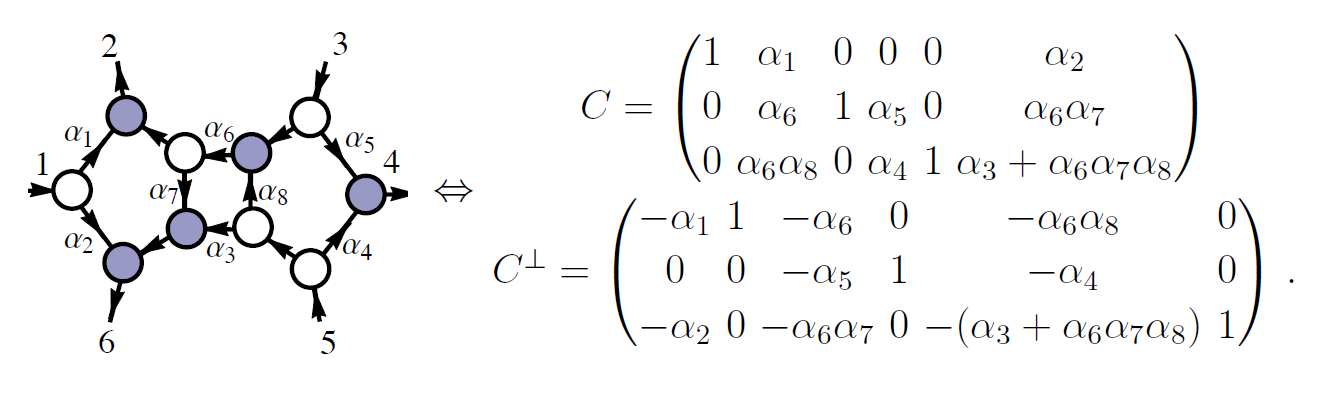
\includegraphics[width=0.9\linewidth]{4+4}
	\caption[4+4]{}
	\label{fig:44}
\end{figure}
We then use the following combination of equation from the $C\cdot\tilde \lambda$ and $C_\perp\cdot \lambda$ delta functions
\begin{equation}
	\begin{aligned}
0=&-\langle 3 4 \rangle + \alpha_{4} \langle 3 5 \rangle
\\
0=&-(\alpha_{5} \langle 3 5 \rangle) + \langle 4 5 \rangle
\\
0=&\left[ 1 2 \right] - \alpha_{2} \left[ 2 6 \right]
\\
0=&\left[ 1 6 \right] + \alpha_{1} \left[ 2 6 \right]
\\
0=&-\left[ 2 3 \right] - \alpha_{5} \left[ 2 4 \right] - \alpha_{6} \alpha_{7} \left[ 2 6 \right]
\\
0=&\alpha_{6} \left[ 2 6 \right] + \left[ 3 6 \right] + \alpha_{5} \left[ 4 6 \right]
\\
0=&-(\alpha_{4} \left[ 2 4 \right]) - \left[ 2 5 \right] - (\alpha_{3} + \alpha_{6} \alpha_{7} \alpha_{8}) \left[ 2 6 \right]
\\
0=&\alpha_{6} \alpha_{8} \left[ 2 6 \right] + \alpha_{4} \left[ 4 6 \right] + \left[ 5 6 \right]
	\end{aligned}
\end{equation}
to obtain
\begin{align*}
	& \alpha_1 = -\frac{[16]}{[26]}\,, \quad \alpha_2 = \frac{[12]}{[26]}\,, \quad \alpha_3 = \frac{\sab{345}}{\aMs{5}{Q_{345}}{6}}\,, \quad \alpha_4 = \frac{\ab{34}}{\ab{35}}\,, \quad
	\alpha_5 = \frac{\ab{45}}{\ab{35}}\,, \\ 
	& \twhite{.}\hspace{1.4cm} 
	\alpha_6 = \frac{\aMs{5}{Q_{345}}{6}}{\ab{35}\sqb{26}}\,, \alpha_7 = -\frac{\aMs{5}{Q_{345}}{2}}{\aMs{5}{Q_{345}}{6}}\,,\quad
	\alpha_8 = - \frac{\aMs{3}{Q_{345}}{6}}{\aMs{5}{Q_{345}}{6}}\,.
\end{align*}
where $Q_{ijk}=p_i+p_j+p_k$
%%%%%%%%%%%%%%%%%%%%%%%%%%%%%%%%%%%%%%%%%%%%%%%%%%%%%%%%%%%%%%%%%%%%%%%%%%%%%%%%%%%%%%%%%%%%%%%%%%%%%%%%%%%%%%%%%%%%%%%%%%%%%%%%%%%%%%%%%%%%%%%%%%%%%%%%%%%%%%%%%%%%%%%%%%%%%%%%
For the other delta functions we get
\begin{equation}
	\begin{aligned}
	 0&=\tilde\eta_1-\frac{[16]}{[26]}\tilde\eta_2+\frac{[12]}{[26]}\tilde\eta_6\\
		0&= \frac{\langle5|Q_{345}|6]}{\expval{35}[26]}\tilde\eta_2+\tilde\eta_3+\frac{\expval{45}}{\expval{35}}\tilde\eta_4-\frac{\langle5|Q_{345}|2]}{\expval{35}[26]}\tilde\eta_6
		\\
		0&= -\frac{\langle3|Q_{45}|6]}{\expval{35}[26]}\tilde\eta_2+\frac{\expval{34}}{\expval{35}}\tilde\eta_4+\tilde\eta_5+\frac{s_{345}\expval{35}[26]+\langle3|Q_{345}|6]\langle5|Q_{345}|2] }{\langle5|Q_{345}|6]}
\tilde\eta_5
	\end{aligned}
\end{equation}
\begin{equation}
	\begin{aligned}
		0&= \frac{\langle5|Q_{345}|6]}{\expval{35}[26]}\tilde\eta_2+\tilde\eta_3+\frac{\expval{45}}{\expval{35}}\tilde\eta_4-\frac{\langle5|Q_{345}|2]}{\expval{35}[26]}\tilde\eta_6
		\\
	\end{aligned}
\end{equation}
\begin{thebibliography}{99}

%\cite{Bjerrum-Bohr:2013bxa}
\bibitem{Bjerrum-Bohr:2013bxa}
N.~E.~J.~Bjerrum-Bohr, J.~F.~Donoghue and P.~Vanhove,
``On-shell Techniques and Universal Results in Quantum Gravity,''
JHEP \textbf{02} (2014), 111
doi:10.1007/JHEP02(2014)111
[arXiv:1309.0804 [hep-th]].
%83 citations counted in INSPIRE as of 21 Aug 2020

%\fi
\end{thebibliography}
\end{document}

